\subsection{یخش پ}
در بخش برای محاسبه ضرایب حلقه هدایت از بهینه‌سازی ازدحام ذرات\LTRfootnote{Particle Swarm Optimization}
استفاده شده است. ضرایب حلقه هدایت بدست آمده در جدول پایین آورده شده است.


\begin{table}[H]
	\caption{ضرایب حلقه هدایت و فاصله ازدست‌دهی }
	\centering
	\begin{tabular}{cc}
	\hline
	Value &  Parameter \\
	\hline
	\lr{95.2874} & \lr{$k_{\epsilon}$}\\
	\lr{50.5153}  & \lr{$k_{\sigma}$}\ \\ 
	\lr{0.5692}& \lr{Miss Distance (m)}  \\
	\hline
\end{tabular}
\end{table}

نتایج شبیه‌سازی در پایین آورده شده است.

\begin{figure}[H]
	\centering
	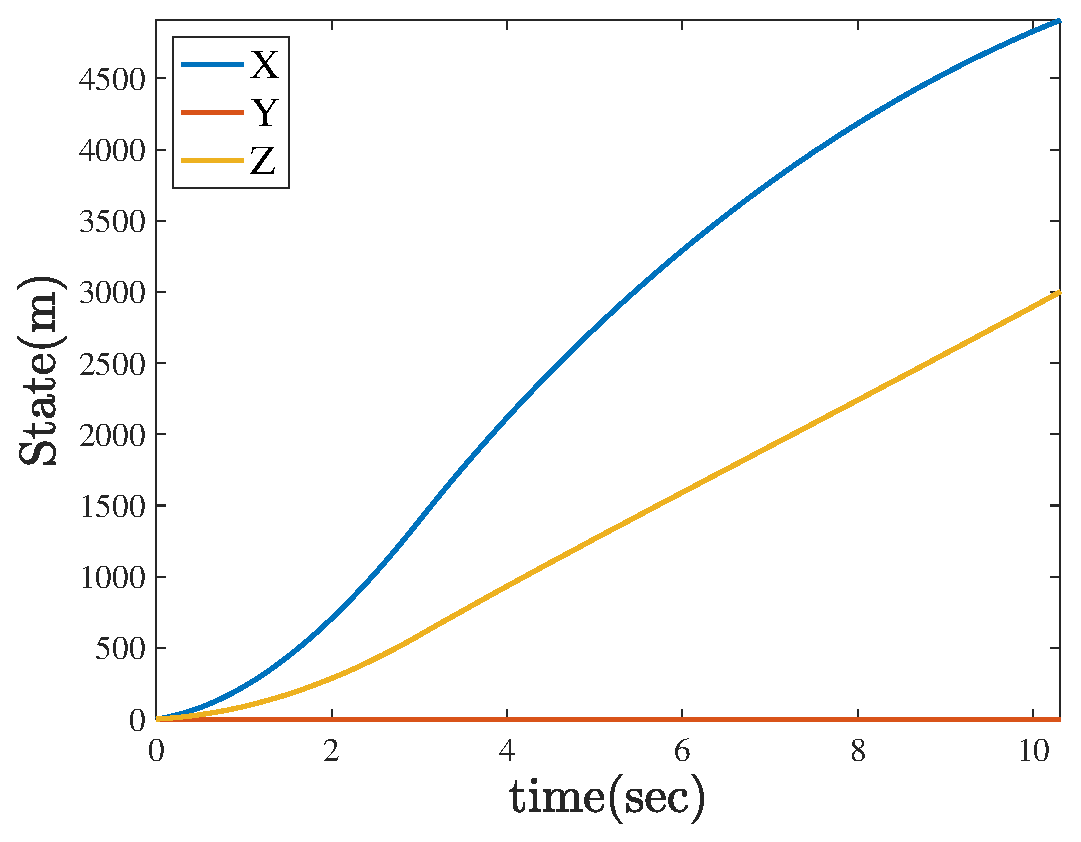
\includegraphics[width=.75\linewidth]{../Figure/c/missle_state}
	\caption{موقعیت موشک در هدایت خط دید پایه}
\end{figure}

\begin{figure}[H]
	\centering
	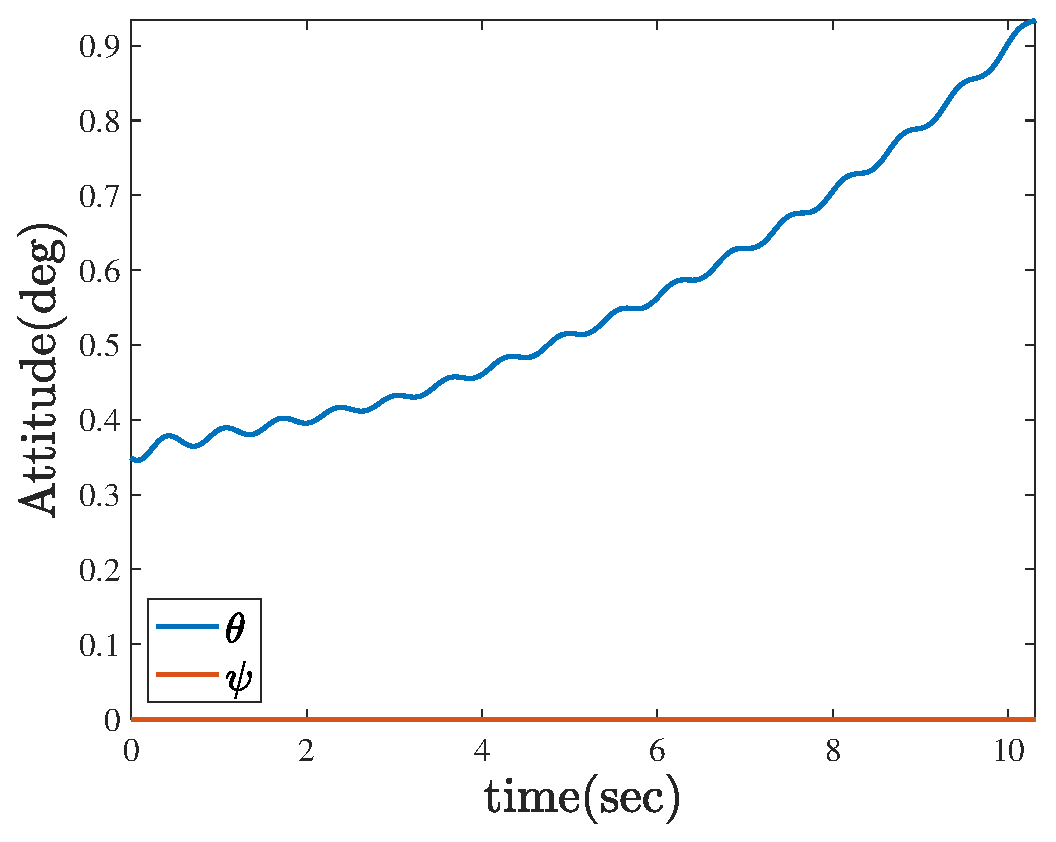
\includegraphics[width=.75\linewidth]{../Figure/c/missle_attitude}
	\caption{وضعیت موشک  در هدایت خط دید پایه}
\end{figure}

\begin{figure}[H]
	\centering
	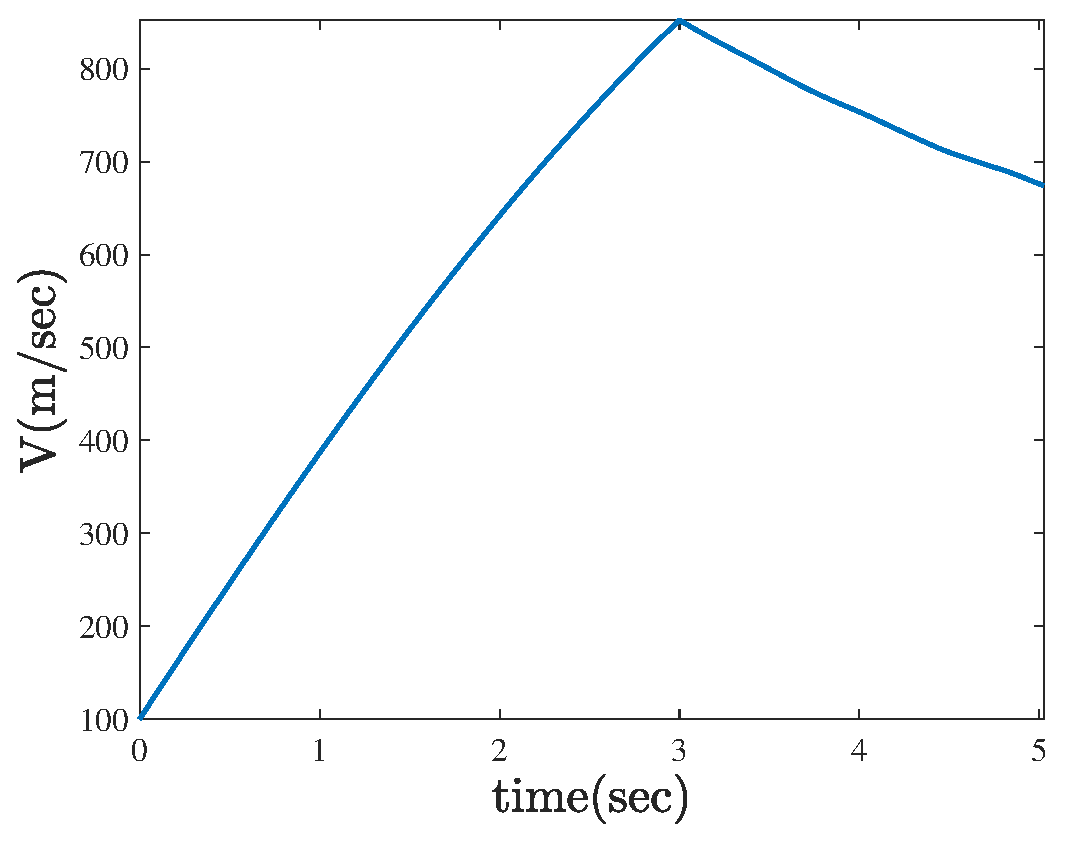
\includegraphics[width=.75\linewidth]{../Figure/c/missle_V}
	\caption{سرعت موشک  در هدایت خط دید پایه}
\end{figure}

\begin{figure}[H]
	\centering
	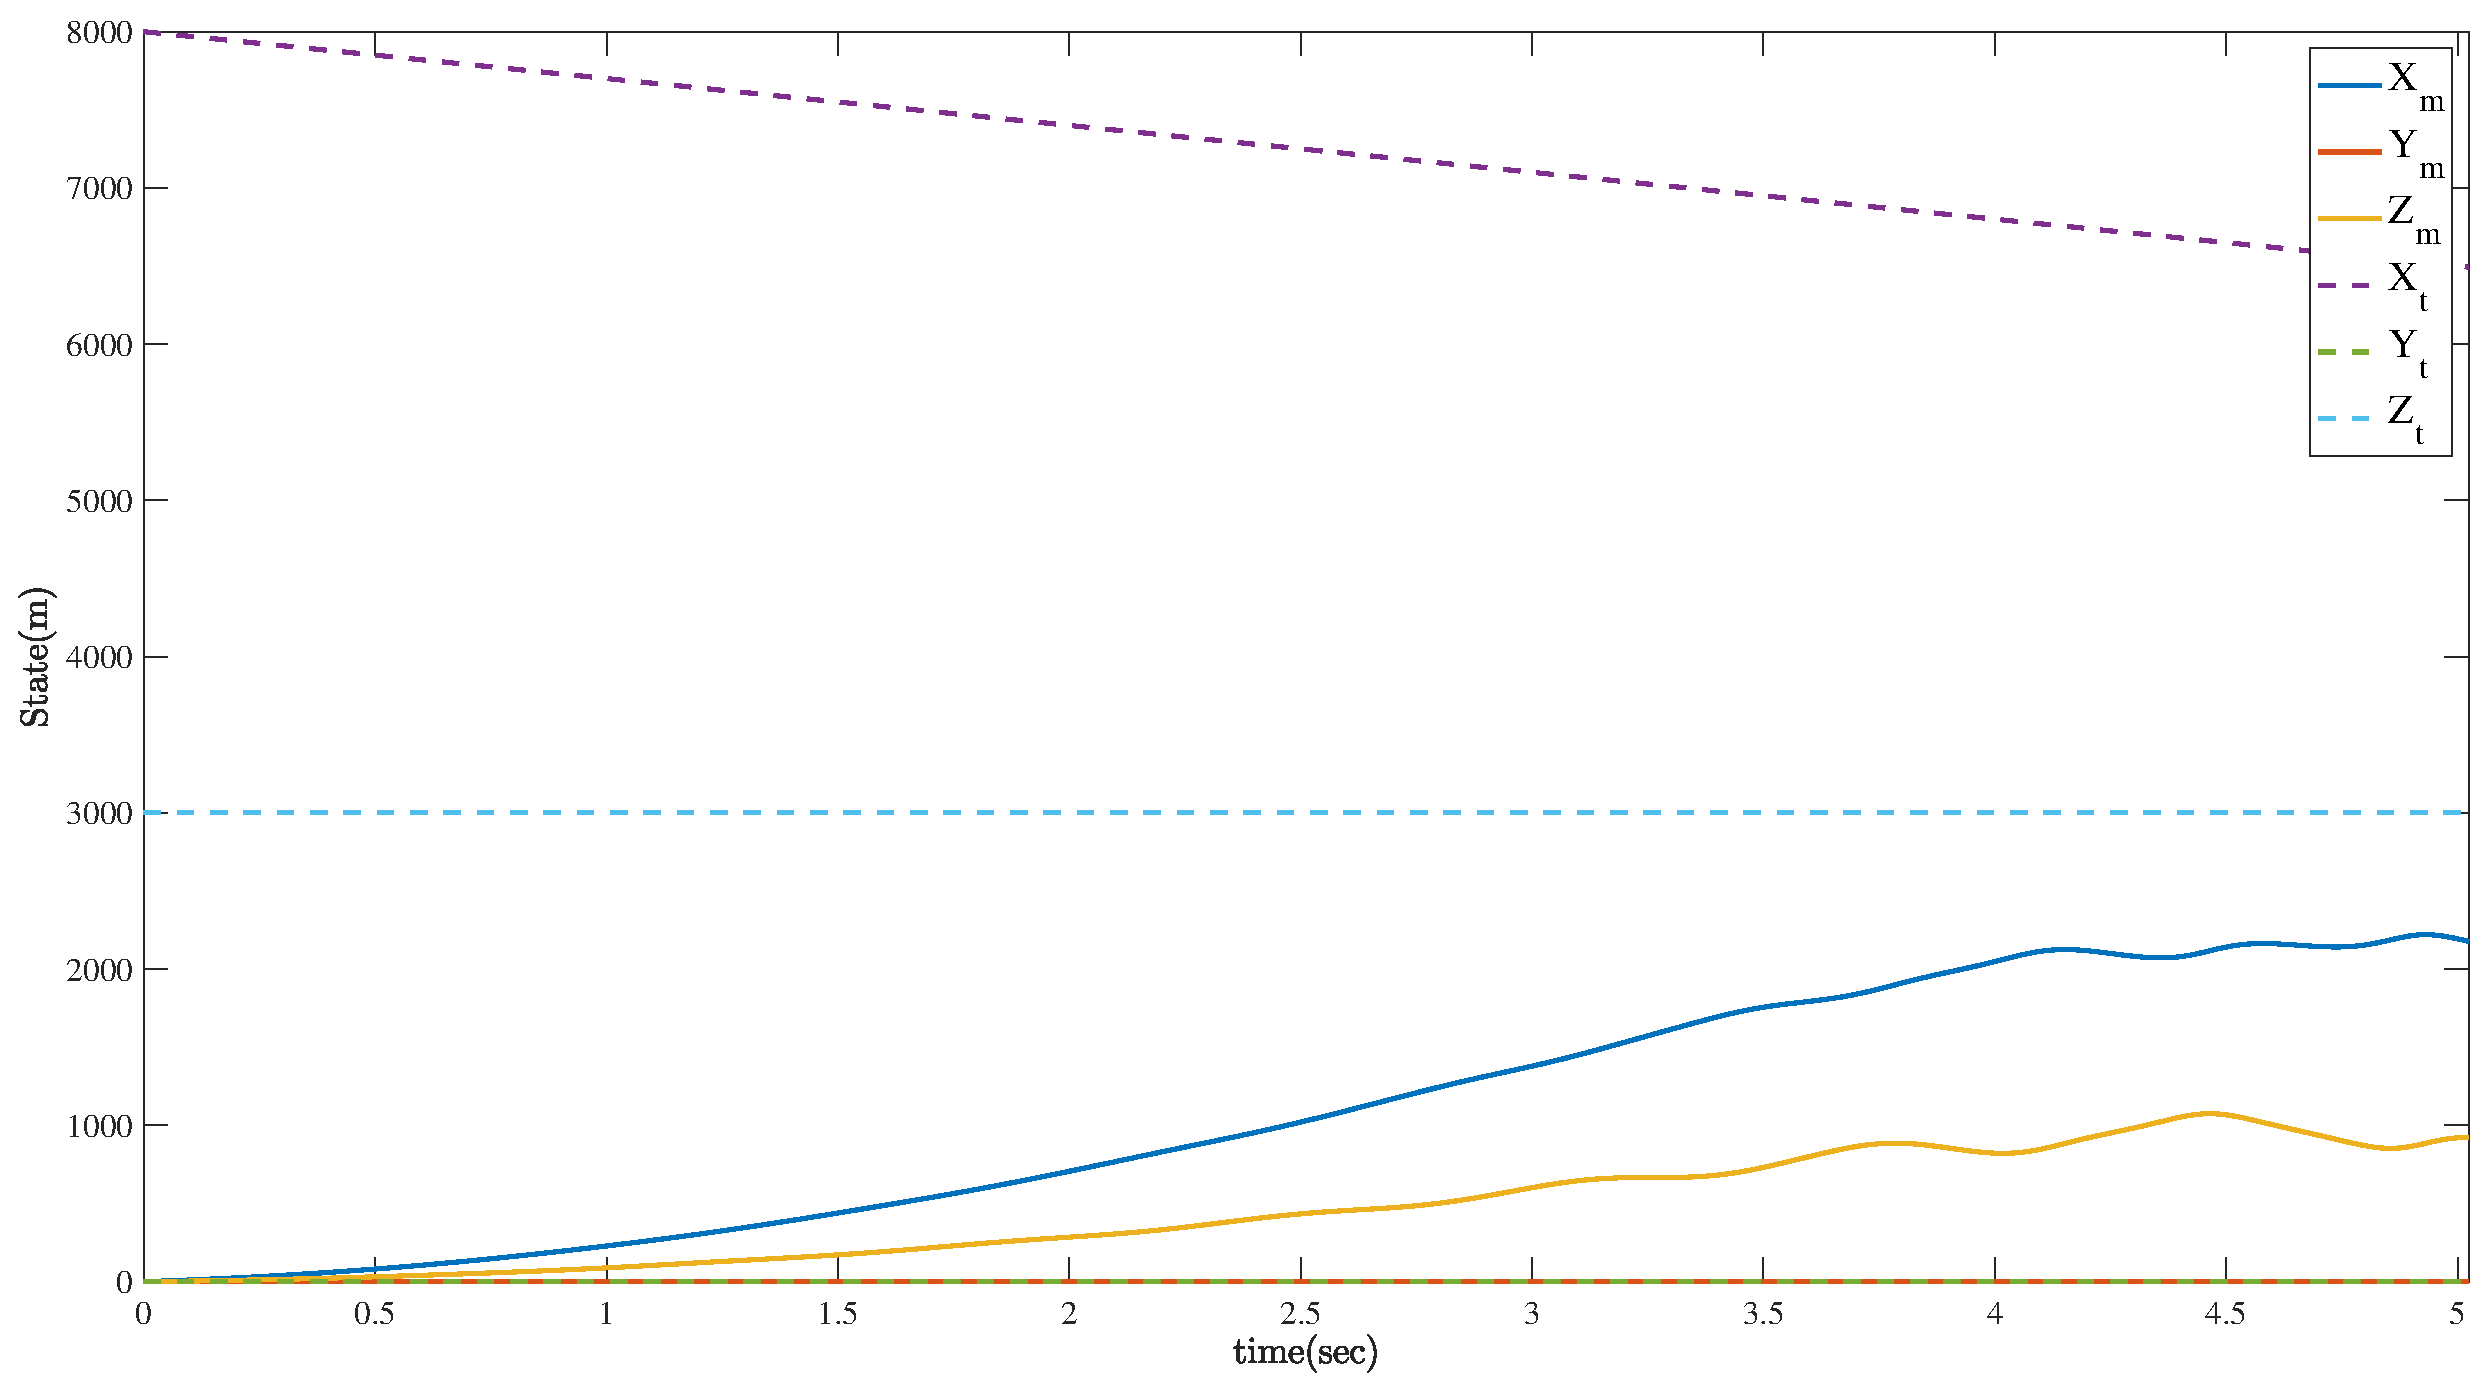
\includegraphics[width=\linewidth]{../Figure/c/missle_vs_target_state}
	\caption{موقعیت موشک و هدف  در هدایت خط دید پایه}
\end{figure}

\begin{figure}[H]
	\centering
	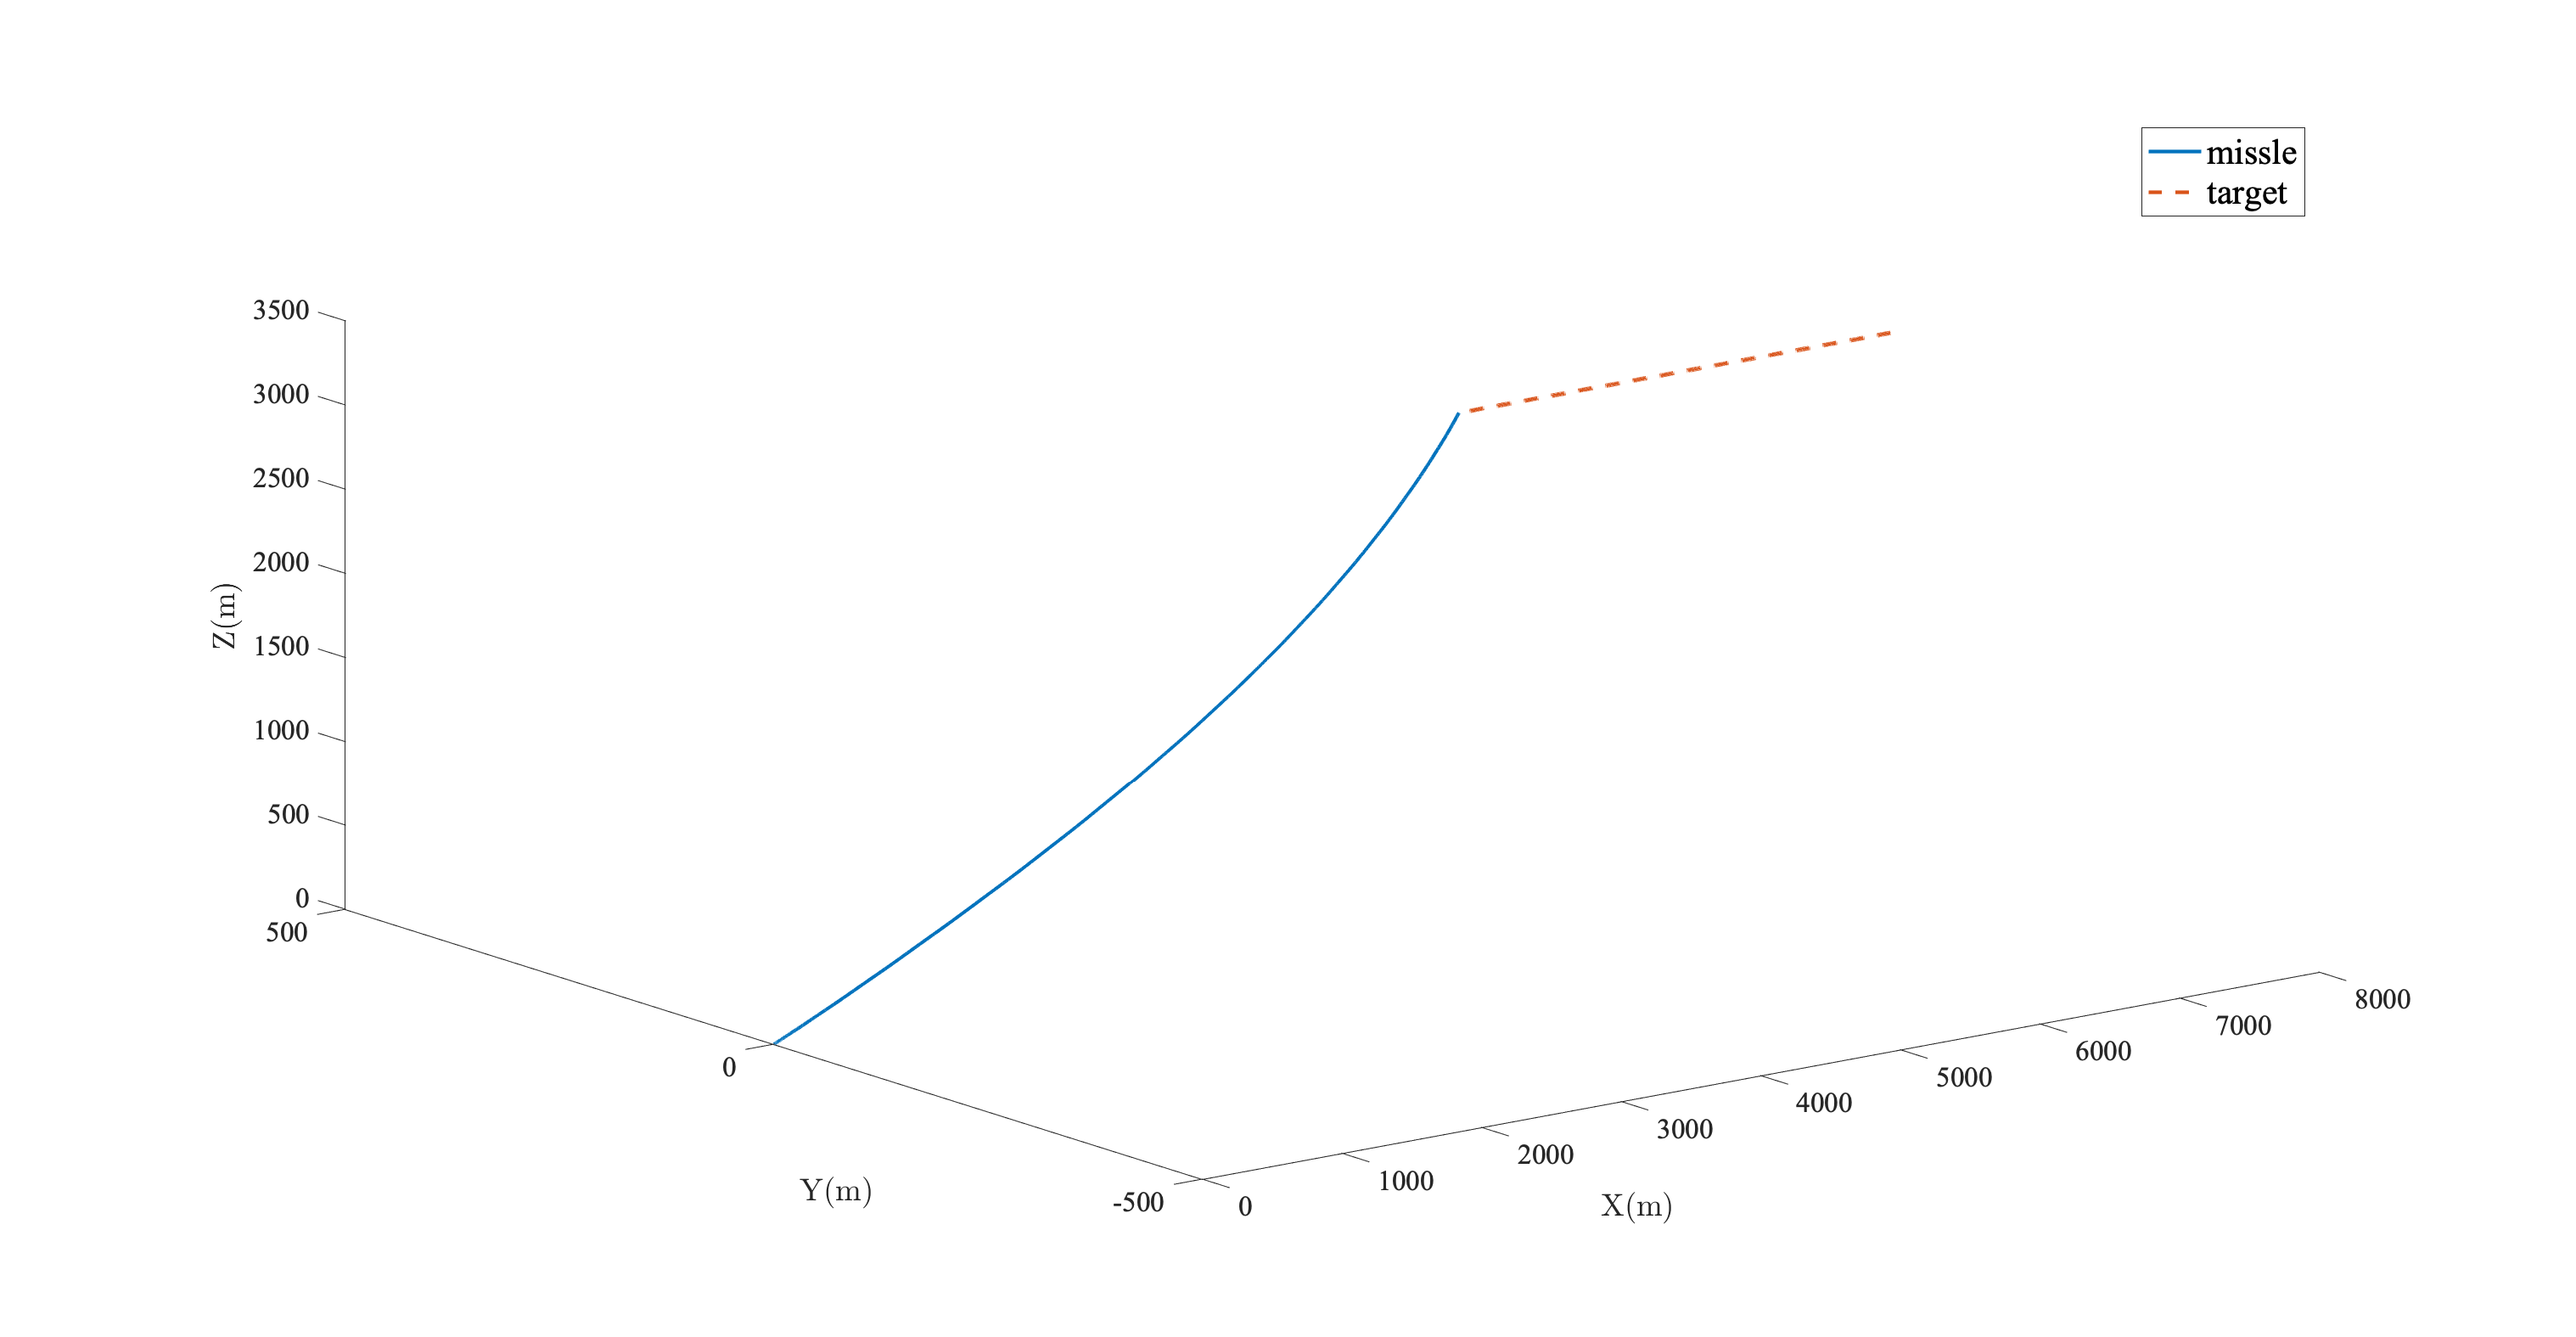
\includegraphics[width=\linewidth]{../Figure/c/3DoF_missle_vs_target_state}
	\caption{موقعیت موشک و هدف به صورت سه بعدی  در هدایت خط دید پایه}
\end{figure}

\begin{figure}[H]
	\centering
	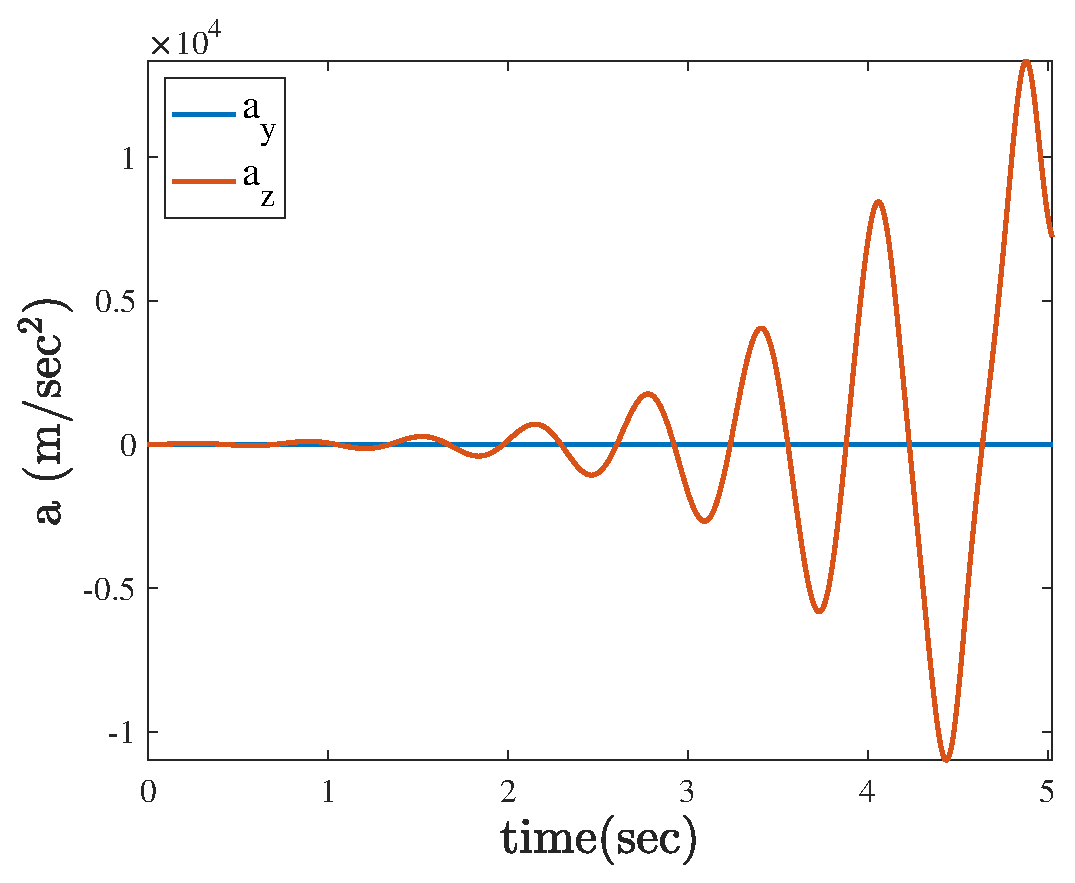
\includegraphics[width=.75\linewidth]{../Figure/c/command}
	\caption{فرمان شتاب در هدایت خط دید پایه}
\end{figure}

\begin{figure}[H]
	\centering
	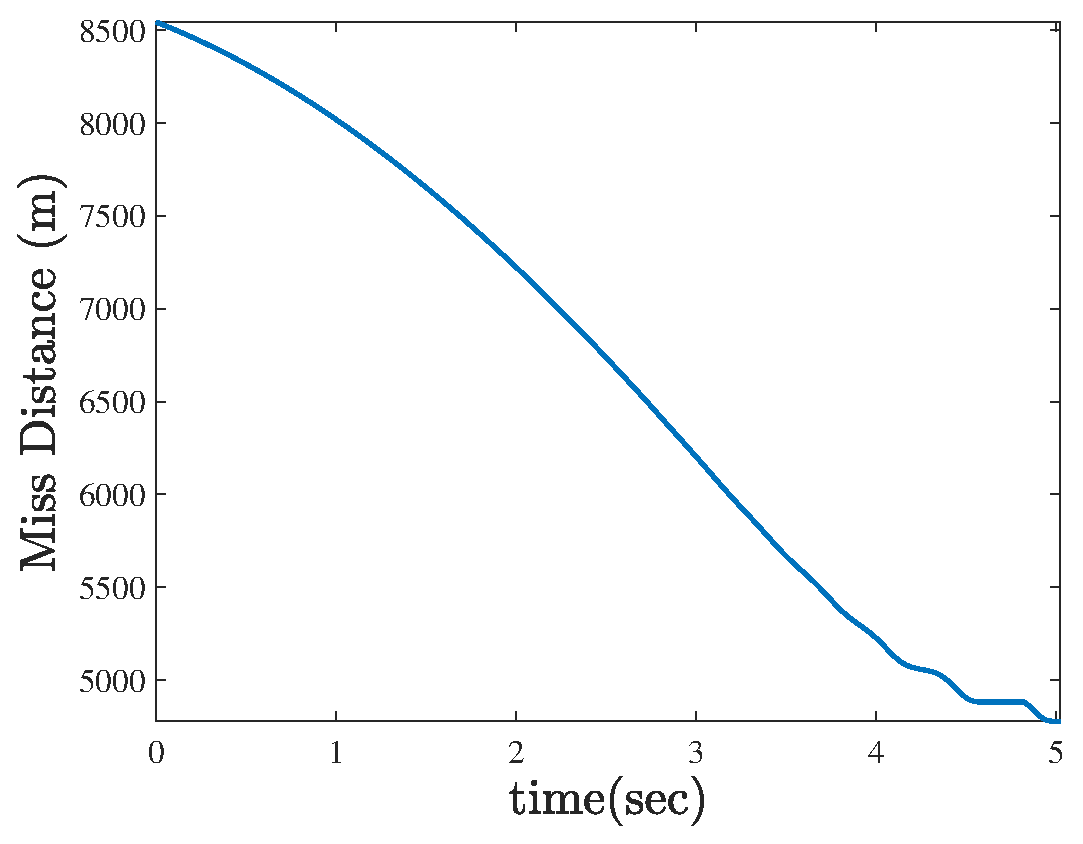
\includegraphics[width=.75\linewidth]{../Figure/c/miss_distance}
	\caption{فاصله ازدست‌دهی در هدایت خط دید پایه}
\end{figure}


